\documentclass[11pt,a4paper]{article}
\usepackage[margin=2.1cm]{geometry}
\usepackage[T1]{fontenc}
\usepackage{lmodern}
\usepackage{microtype}
\usepackage{booktabs}
\usepackage{pgfplots}
\pgfplotsset{compat=1.18}
\usepackage{enumitem}
\usepackage{float}
\usepackage{caption}
\usepackage[hidelinks]{hyperref}
\setlist{nosep, leftmargin=1.4em}
\captionsetup{font=small, labelfont=bf}
\sloppy\emergencystretch=3em

\newcommand{\LossFirst}{10.14}
\newcommand{\LossTrainEnd}{2.199}
\newcommand{\ValFirst}{5.38}
\newcommand{\ValBest}{2.166}
\newcommand{\ValBestStep}{8,250}
\newcommand{\ValPplBest}{8.72}
\newcommand{\ValPoints}{33}
\newcommand{\LastStep}{8,380}
\newcommand{\MaxSteps}{9,134}
\newcommand{\DonePct}{91.7\%}
\newcommand{\TokensSeen}{2.20B}
\newcommand{\Gap}{+0.001}
\newcommand{\ValSlope}{-0.023}
\newcommand{\GradMed}{0.23}
\newcommand{\GradMax}{2.60}
\newcommand{\GradSpikes}{35}
\newcommand{\Tps}{33,458}
\newcommand{\PeakMem}{9.2}
\newcommand{\ProbeN}{10}
\newcommand{\ProbeGreedy}{3}
\newcommand{\ProbeSample}{17\%}
\newcommand{\ProbeAgree}{6}
\newcommand{\ProbeLoops}{4}
\newcommand{\ProbeSame}{10}
\newcommand{\OrderN}{400}
\newcommand{\OrderSame}{100.0\%}
\newcommand{\OrderAccA}{31.0\%}
\newcommand{\OrderAccB}{31.0\%}
\newcommand{\RelDiff}{1.17\%}
\newcommand{\RepeatDiff}{0}
\newcommand{\CpuDiff}{2.2e-05}
\newcommand{\CpuArgmax}{100.0\%}
\newcommand{\Params}{100.1M}
\newcommand{\EvalItems}{3,544}
\newcommand{\EvalAcc}{26.9\%}
\newcommand{\EvalChance}{24.8\%}
\newcommand{\EvalExcluded}{75}
\newcommand{\LoopsGreedy}{56}
\newcommand{\LoopsSampled}{4}
\newcommand{\LoopTexts}{102}


\title{\textbf{PRANA-G 100M: Checkpoint Analysis Report}}
\author{Namit Aggarwal, PRANA-G AI}
\date{3 November 2026}

\begin{document}
\maketitle

\noindent Checkpoint \texttt{ckpt\_best.pt} (step \ValBestStep, \Params{} parameters, 12 layers, hidden size 768) from the 100M training run on an
A100 MIG slice, trained on 17 domains. All 34 training and validation files used here were checked against the run's preflight log and match it
token for token. Every number below comes from the result files in \texttt{results/}; \S\ref{sec:repro} gives the one command that reproduces them.

\section{Training and validation loss}
\begin{figure}[H]\centering
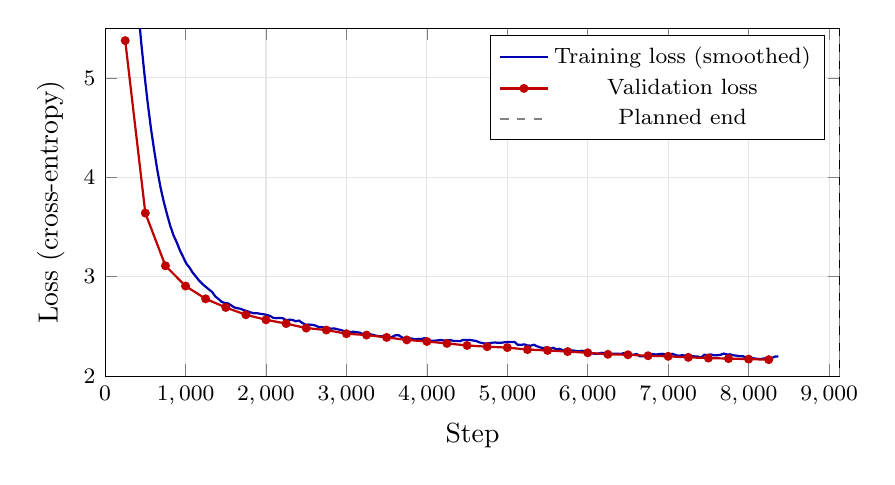
\begin{tikzpicture}
\begin{axis}[width=0.9\linewidth, height=6cm, xlabel={Step}, ylabel={Loss (cross-entropy)}, ymin=2, ymax=5.5,
  xmin=0, xmax=9134, legend style={font=\footnotesize}, tick label style={font=\footnotesize},
  scaled x ticks=false, xticklabel style={/pgf/number format/1000 sep={,}}, grid=major, grid style={gray!20}]
\addplot[blue!70!black, thick] coordinates {(130,8.8980) (170,8.3404) (210,7.8047) (250,7.3052) (290,6.8520) (330,6.4415) (370,6.0591) (410,5.7002) (450,5.3473) (490,5.0297) (530,4.7452) (570,4.4913) (610,4.2722) (650,4.0687) (690,3.8935) (730,3.7510) (770,3.6272) (810,3.5117) (850,3.4166) (890,3.3467) (930,3.2649) (970,3.1986) (1010,3.1317) (1050,3.0915) (1090,3.0396) (1130,3.0008) (1170,2.9592) (1210,2.9272) (1250,2.8989) (1290,2.8720) (1330,2.8469) (1370,2.8018) (1410,2.7759) (1450,2.7461) (1490,2.7355) (1530,2.7311) (1570,2.7105) (1610,2.6899) (1650,2.6827) (1690,2.6752) (1730,2.6624) (1770,2.6524) (1810,2.6404) (1850,2.6329) (1890,2.6332) (1930,2.6267) (1970,2.6223) (2010,2.6159) (2050,2.6058) (2090,2.5862) (2130,2.5831) (2170,2.5856) (2210,2.5822) (2250,2.5630) (2290,2.5678) (2330,2.5652) (2370,2.5519) (2410,2.5588) (2450,2.5360) (2490,2.5177) (2530,2.5185) (2570,2.5165) (2610,2.5101) (2650,2.4954) (2690,2.4931) (2730,2.4875) (2770,2.4822) (2810,2.4776) (2850,2.4797) (2890,2.4709) (2930,2.4643) (2970,2.4535) (3010,2.4348) (3050,2.4446) (3090,2.4459) (3130,2.4417) (3170,2.4371) (3210,2.4198) (3250,2.4172) (3290,2.4226) (3330,2.4146) (3370,2.4062) (3410,2.4026) (3450,2.3998) (3490,2.3968) (3530,2.3829) (3570,2.3957) (3610,2.4111) (3650,2.4113) (3690,2.3900) (3730,2.3740) (3770,2.3758) (3810,2.3784) (3850,2.3705) (3890,2.3739) (3930,2.3730) (3970,2.3823) (4010,2.3702) (4050,2.3557) (4090,2.3555) (4130,2.3594) (4170,2.3632) (4210,2.3588) (4250,2.3594) (4290,2.3642) (4330,2.3526) (4370,2.3543) (4410,2.3515) (4450,2.3638) (4490,2.3630) (4530,2.3642) (4570,2.3589) (4610,2.3541) (4650,2.3404) (4690,2.3323) (4730,2.3270) (4770,2.3298) (4810,2.3364) (4850,2.3378) (4890,2.3350) (4930,2.3364) (4970,2.3409) (5010,2.3438) (5050,2.3421) (5090,2.3437) (5130,2.3155) (5170,2.3143) (5210,2.3193) (5250,2.3085) (5290,2.3061) (5330,2.3155) (5370,2.2999) (5410,2.2881) (5450,2.2827) (5490,2.2892) (5530,2.2712) (5570,2.2853) (5610,2.2693) (5650,2.2745) (5690,2.2604) (5730,2.2482) (5770,2.2590) (5810,2.2583) (5850,2.2540) (5890,2.2489) (5930,2.2554) (5970,2.2431) (6010,2.2356) (6050,2.2296) (6090,2.2244) (6130,2.2259) (6170,2.2346) (6210,2.2305) (6250,2.2256) (6290,2.2254) (6330,2.2265) (6370,2.2251) (6410,2.2233) (6450,2.2315) (6490,2.2275) (6530,2.2124) (6570,2.2155) (6610,2.2223) (6650,2.1992) (6690,2.2005) (6730,2.1972) (6770,2.2179) (6810,2.2217) (6850,2.2170) (6890,2.2222) (6930,2.2242) (6970,2.2170) (7010,2.2127) (7050,2.2248) (7090,2.2128) (7130,2.2047) (7170,2.2100) (7210,2.2077) (7250,2.1982) (7290,2.1998) (7330,2.1987) (7370,2.1962) (7410,2.1881) (7450,2.2146) (7490,2.2115) (7530,2.2185) (7570,2.2086) (7610,2.2104) (7650,2.2145) (7690,2.2266) (7730,2.2180) (7770,2.2192) (7810,2.2092) (7850,2.2062) (7890,2.1988) (7930,2.2004) (7970,2.1851) (8010,2.1744) (8050,2.1803) (8090,2.1760) (8130,2.1711) (8170,2.1746) (8210,2.1796) (8250,2.1715) (8290,2.1826) (8330,2.1970) (8370,2.1968)};
\addplot[red!75!black, thick, mark=*, mark size=1.2pt] coordinates {(250,5.3755) (500,3.6406) (750,3.1100) (1000,2.9062) (1250,2.7775) (1500,2.6910) (1750,2.6172) (2000,2.5669) (2250,2.5286) (2500,2.4835) (2750,2.4636) (3000,2.4267) (3250,2.4131) (3500,2.3895) (3750,2.3643) (4000,2.3482) (4250,2.3290) (4500,2.3084) (4750,2.2960) (5000,2.2869) (5250,2.2670) (5500,2.2586) (5750,2.2468) (6000,2.2349) (6250,2.2194) (6500,2.2149) (6750,2.2049) (7000,2.1993) (7250,2.1887) (7500,2.1817) (7750,2.1766) (8000,2.1710) (8250,2.1656)};
\addplot[gray, dashed] coordinates {(9134,2) (9134,5.5)};
\legend{Training loss (smoothed), Validation loss, Planned end}
\end{axis}
\end{tikzpicture}

\caption{Training loss (smoothed) and validation loss on the mixed validation set, every 250 steps.}
\end{figure}

\begin{table}[H]\centering\small
\begin{tabular}{ll}
\toprule
Training loss, first logged step / end (smoothed) & \LossFirst{} / \LossTrainEnd \\
Validation loss, first evaluation (step 250) / best & \ValFirst{} / \ValBest{} at step \ValBestStep{} (perplexity \ValPplBest) \\
Training minus validation loss at the end & \Gap{} \\
Validation loss change over the last 1,000 steps & \ValSlope{} per 1,000 steps \\
Steps completed & \LastStep{} of \MaxSteps{} planned (\DonePct), \TokensSeen{} tokens \\
Gradient norm (median / max) & \GradMed{} / \GradMax{}; \GradSpikes{} spikes above 3$\times$ median \\
Throughput, peak memory & \Tps{} tokens/s, \PeakMem{} GB \\
\bottomrule
\end{tabular}
\caption{Loss summary (from \texttt{metrics.jsonl}).}
\end{table}

\begin{itemize}
\item \textbf{No overfitting.} Training and validation loss are equal at the end (difference \Gap), so the model is not memorising its data.
\item \textbf{Not converged.} Validation loss was still falling (\ValSlope{} per 1,000 steps) when the run stopped; more tokens would still help.
\item \textbf{The run did not finish.} It stopped at step \LastStep{} of \MaxSteps{} when the GPU slot ended. The last checkpoint was saved at
  step 8,250, so the final 130 steps were lost.
\item \textbf{Training was stable.} All losses are finite. Almost all gradient-norm spikes happened in the first 400 steps (warm-up); after step 1,000
  there were only two small ones (1.76 at step 1,810 and 0.95 at step 4,180).
\end{itemize}

\section{Domain-wise perplexity and next-token prediction}
Each domain's validation file was cut into the same non-overlapping 2,048-token windows (100 windows, about 200k tokens; astronomy and finance
have fewer). For every position the model predicts the next token: \emph{cross-entropy} is the average loss, \emph{perplexity} is $e$ raised to the cross-entropy, \emph{top-1}/\emph{top-5} is how often the true token is the model's first choice / among its five most likely,
and \emph{calibration error} is the gap between how confident the model is and how often it is right.

\begin{table}[H]\centering\small
\begin{tabular}{lrrrrrr}
\toprule
Domain & Tokens & Cross-entropy & Perplexity & Top-1 & Top-5 & Calibration error \\
\midrule
cad & 204,800 & 0.217 & 1.24 & 94.7\% & 98.2\% & 0.2\% \\
code & 204,800 & 1.276 & 3.58 & 74.0\% & 87.6\% & 0.8\% \\
bio & 204,800 & 1.306 & 3.69 & 73.7\% & 85.1\% & 0.8\% \\
finance & 86,016 & 1.363 & 3.91 & 73.8\% & 81.7\% & 4.7\% \\
engineering & 204,800 & 1.440 & 4.22 & 70.3\% & 84.6\% & 0.5\% \\
scidisc & 204,800 & 1.566 & 4.79 & 67.6\% & 81.4\% & 0.4\% \\
sciprog & 204,800 & 1.732 & 5.65 & 65.6\% & 82.6\% & 1.2\% \\
multistep & 204,800 & 1.883 & 6.58 & 59.8\% & 75.7\% & 0.8\% \\
earth & 204,800 & 1.938 & 6.95 & 63.2\% & 77.4\% & 0.3\% \\
gen\_eng & 204,800 & 2.349 & 10.47 & 53.0\% & 73.7\% & 1.2\% \\
sciqa & 204,800 & 2.432 & 11.38 & 50.8\% & 72.7\% & 0.9\% \\
chem & 204,800 & 2.445 & 11.53 & 50.3\% & 72.1\% & 0.6\% \\
exp\_val & 204,800 & 2.635 & 13.94 & 49.4\% & 69.4\% & 0.7\% \\
physics & 204,800 & 2.750 & 15.65 & 46.0\% & 67.5\% & 0.3\% \\
math & 204,800 & 2.773 & 16.00 & 47.2\% & 67.8\% & 0.8\% \\
astro & 100,352 & 2.983 & 19.74 & 42.9\% & 64.8\% & 0.6\% \\
tech\_comm & 204,800 & 3.108 & 22.38 & 43.9\% & 63.0\% & 0.6\% \\
\bottomrule
\end{tabular}

\caption{Next-token prediction for all 17 training domains, sorted by perplexity.}
\end{table}

\begin{itemize}
\item \textbf{Very low perplexity points to templated data.} CAD (perplexity 1.24, top-1 95\%) is almost fully predictable, and code, biology and
  finance (3.6--3.9) are also unusually easy. Text this predictable is usually generated from templates or highly repetitive; such data teaches
  the model little and should be checked for diversity before the 30B run.
\item \textbf{The hardest domains are technical communication, astronomy, maths and physics} (perplexity 16--22, top-1 43--47\%), which are also the
  most varied natural text.
\item Multi-step reasoning is easy at the token level (perplexity 6.6) but the model solves almost no problems (\S\ref{sec:bench}): predicting
  the style of a worked solution is not the same as solving it.
\item Calibration is good: below 1.5\% error in every domain except finance (4.7\%), so the model's confidence matches how often it is right.
\end{itemize}

\section{Generation quality, repetition and consistency}
\paragraph{Probes.} Ten fixed one-line prompts with an automatic check, answered greedily and with three seeded samples (temperature 0.8).

\begin{table}[H]\centering\small
\begin{tabular}{llccc}
\toprule
Domain & Prompt & Greedy & Samples passing & Loop \\
\midrule
arithmetic & \texttt{Question: What is 17 * 24? Answer:} & fail & 0/3 & no \\
arithmetic & \texttt{Question: What is 125 + 379? Answer:} & fail & 0/3 & no \\
math & \texttt{The derivative of x\textasciicircum{}2 with respect to x is} & pass & 1/3 & no \\
code & \texttt{def add(a, b):     return} & pass & 2/3 & no \\
code & \texttt{def factorial(n):     if n == 0:         ret} & fail & 0/3 & yes \\
chemistry & \texttt{The chemical formula of water is} & fail & 0/3 & yes \\
physics & \texttt{Newton's second law of motion states that} & pass & 1/3 & no \\
physics & \texttt{The speed of light in vacuum is approximatel} & fail & 0/3 & yes \\
biology & \texttt{DNA is made of four nucleotides:} & fail & 1/3 & yes \\
earth & \texttt{The three main types of rock are} & fail & 0/3 & no \\
\bottomrule
\end{tabular}

\caption{Probe results. ``Loop'' means the greedy answer keeps repeating itself.}
\end{table}

\noindent The automatic check passes \ProbeGreedy{} of \ProbeN{} greedy answers, but reading them, only \texttt{def add(a, b): return a + b} is
really correct: the physics answer matched the word ``force'' in a wrong statement, and the maths answer matched ``2x'' inside unrelated algebra.
Wrong facts are stated confidently (``the speed of light in vacuum is approximately 1.5 times the speed of light'').

\paragraph{Repetition: greedy decoding against sampling.} Six held-out documents per domain were cut after 64 tokens and continued for 96 tokens,
once greedily and once with a seeded sample (temperature 0.8). The table shows the share of repeated 4-grams and the number of continuations that
fall into a loop.

\begin{table}[H]\centering\small
\begin{tabular}{lrrrrrr}
\toprule
Domain & Texts & Real text & Greedy & Greedy loops & Sampled (T=0.8) & Sampled loops \\
\midrule
math & 6 & 5\% & 64\% & 6 & 5\% & 0 \\
physics & 6 & 1\% & 32\% & 1 & 5\% & 0 \\
chem & 6 & 2\% & 68\% & 6 & 16\% & 0 \\
bio & 6 & 5\% & 18\% & 1 & 4\% & 0 \\
earth & 6 & 1\% & 30\% & 2 & 6\% & 0 \\
scidisc & 6 & 2\% & 53\% & 4 & 9\% & 0 \\
sciqa & 6 & 5\% & 40\% & 3 & 12\% & 0 \\
sciprog & 6 & 16\% & 70\% & 6 & 23\% & 2 \\
code & 6 & 16\% & 55\% & 4 & 22\% & 2 \\
cad & 6 & 16\% & 15\% & 0 & 16\% & 0 \\
multistep & 6 & 0\% & 0\% & 0 & 0\% & 0 \\
astro & 6 & 2\% & 49\% & 4 & 2\% & 0 \\
finance & 6 & 8\% & 41\% & 4 & 9\% & 0 \\
engineering & 6 & 0\% & 6\% & 0 & 1\% & 0 \\
gen\_eng & 6 & 4\% & 57\% & 4 & 4\% & 0 \\
exp\_val & 6 & 1\% & 63\% & 5 & 7\% & 0 \\
tech\_comm & 6 & 1\% & 72\% & 6 & 1\% & 0 \\
\midrule All & 102 & & & 56 & & 4 \\
\bottomrule
\end{tabular}

\caption{Repeated 4-grams in the real continuation, in greedy output and in sampled output, and repetition loops.}
\end{table}

\noindent \textbf{Most of the looping comes from greedy decoding.} Greedy continuations loop in \LoopsGreedy{} of \LoopTexts{} texts; sampled
continuations of the same prompts loop in only \LoopsSampled, and repeat about as much as real text. Greedy decoding always takes the single most
likely token, and a small model's most likely continuation is often the text it has just written. Evaluation and demos should therefore use
sampling (or a repetition penalty), and SFT must still teach the model to stop.

\paragraph{Consistency.}
\begin{itemize}
\item Greedy decoding gives identical text when repeated (\ProbeSame/\ProbeN{} probes).
\item The three samples agree with each other on \ProbeAgree{} of \ProbeN{} probes, mostly because they all fail; correct answers are not stable across samples.
\item The two checkpoints 50 steps apart give the same benchmark answer on 91.7\% of questions, and their overall accuracy differs by
  0.06 points (26.9\% and 26.9\%).
\item Scorer check: reversing the order of the options changed none of \OrderN{} multiple-choice answers, so the benchmark cannot favour a position.
\end{itemize}

\section{Checkpoint integrity and reproducibility}
\begin{table}[H]\centering\small
\begin{tabular}{lll}
\toprule
Check & \texttt{ckpt\_best.pt} & \texttt{ckpt\_last.pt} \\
\midrule
File size & 1.20 GB & 1.20 GB \\
SHA-256 (first 16) & \texttt{54252dfec6573c82} & \texttt{2b72125a3bdb2caf} \\
Step & 8,250 & 8,200 \\
Parameters & 100,092,672 & 100,092,672 \\
Tensors & 110 & 110 \\
All weights finite & yes & yes \\
Tokenizer hash matches & yes & yes \\
Optimizer state saved & yes & yes \\
Validation loss stored & 2.1656 & -- \\
Matches metrics.jsonl & yes & -- \\
Saved with PyTorch & 2.10.0+cu128 & 2.10.0+cu128 \\
\bottomrule
\end{tabular}

\caption{Integrity of the two checkpoints.}
\end{table}

\begin{itemize}
\item Both files load, all weights are finite, the tokenizer hash matches, and the validation loss stored in \texttt{ckpt\_best.pt} equals the value in
  the training log exactly.
\item \textbf{Why the validation loss was reported as null.} Validation loss is measured every 250 steps, but checkpoints are saved every 200 steps.
  \texttt{ckpt\_last.pt} is from step 8,200, which is not an evaluation step, so it has no validation loss stored, and the sample-output script printed
  it as null. \texttt{ckpt\_best.pt} (step 8,250) has it: 2.166. Nothing is missing from the training itself. Note that \texttt{ckpt\_last.pt} is
  50 steps \emph{older} than \texttt{ckpt\_best.pt}, because the run stopped after step 8,250's save.
\item The two checkpoints have the same configuration and tensors and differ by \RelDiff{} of their weights (50 steps of training).
\item Repeating a forward pass gives identical outputs (max difference \RepeatDiff); CPU and Apple-GPU outputs differ by at most \CpuDiff{} and
  predict the same token at every position (\CpuArgmax).
\item The benchmark re-scores its first 20 questions on every run and requires identical answers; this passed on every run. The whole analysis
  was produced by one command (\S\ref{sec:repro}).
\end{itemize}

\section{Re-evaluation of the benchmark}\label{sec:bench}
The benchmark is frozen at version 2.1: 3,619 questions in 19 domains (the first set of 2,340 questions, of which 2,337 were scored in the first report,
plus biology, astronomy, finance, earth science, scientific discovery, scientific programming and CAD), with a SHA-256 hash for every file.

\paragraph{Leakage.} Every question was searched for in all 17 training files. 75 were found and removed from scoring, leaving \EvalItems.
39 are in \texttt{sciqa.train.bin}, which contains maths questions with worked answers that include MMLU high-school maths questions
word for word (median match 95\%); 28 are in \texttt{math.train.bin} (forum copies), and 8 in physics, technical communication and chemistry.
Maths is hit hardest: 55 of its 400 questions were removed. The \texttt{sciqa} text also carries leftover source tags (``GSM\_AnsAug'',
``Expected Answer:''), like the multistep data.

\paragraph{Results.} Overall accuracy is \EvalAcc{} against \EvalChance{} for random guessing.

\begin{table}[H]\centering\small
\begin{tabular}{lrrcrc}
\toprule
Domain & $n$ & Accuracy & 95\% CI & Chance & Above chance \\
\midrule
astro & 150 & 32.7\% & 25.7\%--40.5\% & 25.0\% & yes \\
bio & 290 & 25.5\% & 20.8\%--30.8\% & 25.0\% & no \\
cad & 1 & 0.0\% & 0.0\%--79.3\% & 25.0\% & no \\
chemistry & 252 & 25.8\% & 20.8\%--31.5\% & 24.5\% & no \\
code & 202 & 24.8\% & 19.3\%--31.1\% & 25.0\% & no \\
earth & 274 & 32.1\% & 26.9\%--37.9\% & 25.0\% & yes \\
electrical\_eng & 143 & 32.2\% & 25.1\%--40.2\% & 25.0\% & yes \\
engineering & 40 & 12.5\% & 5.5\%--26.1\% & 18.8\% & no \\
exp\_val & 24 & 20.8\% & 9.2\%--40.5\% & 19.8\% & no \\
finance & 358 & 24.6\% & 20.4\%--29.3\% & 25.0\% & no \\
math & 345 & 22.3\% & 18.2\%--27.0\% & 25.0\% & no \\
multistep & 200 & 1.5\% & 0.5\%--4.3\% & 0.0\% & yes \\
physics & 409 & 25.9\% & 21.9\%--30.4\% & 24.7\% & no \\
scidisc & 200 & 50.0\% & 43.1\%--56.9\% & 50.0\% & no \\
sciml & 16 & 25.0\% & 10.2\%--49.5\% & 25.0\% & no \\
sciprog & 4 & 25.0\% & 4.6\%--69.9\% & 25.0\% & no \\
sciqa & 599 & 30.4\% & 26.8\%--34.2\% & 25.0\% & yes \\
simulation & 22 & 31.8\% & 16.4\%--52.7\% & 25.0\% & no \\
tech\_comm & 15 & 33.3\% & 15.2\%--58.3\% & 25.0\% & no \\
\bottomrule
\end{tabular}

\caption{Benchmark accuracy by domain (multiple choice: random guessing 25\%, PubMedQA yes/no 50\%; GSM8K numeric: 0\%).}
\end{table}

\begin{itemize}
\item \textbf{Above chance:} school science (sciqa 30.4\%), earth science (32.1\%), astronomy (32.7\%) and electrical engineering (32.2\%).
  Multistep is formally above chance only because its chance level is 0 (3 of 200 solved).
\item \textbf{At chance:} maths, physics, chemistry, biology, finance, code and every hand-written PRANA-G domain.
\item \textbf{Scientific discovery:} the model answers ``yes'' to all 200 PubMedQA questions whatever the abstract says (50\%).
\end{itemize}

\section{Scientific capability gap analysis}
The table maps the 20 domains of the 30B token plan to what the 100M run trained on, its benchmark result and its validation perplexity.

\begin{table}[H]\centering\scriptsize
\begin{tabular}{lrrp{4.7cm}rp{2.9cm}}
\toprule
Domain (30B plan) & Plan & 100M run & Benchmark accuracy & Val.\ ppl & Status \\
\midrule
Mathematics & 2.4B & 0.395B & math 22\% (ch.\ 25\%, $n$=345) & 16.0 & at chance \\
Physics & 2.1B & 0.209B & physics 26\% (ch.\ 25\%, $n$=409) & 15.6 & at chance \\
Chemistry & 1.2B & 0.070B & chemistry 26\% (ch.\ 25\%, $n$=252) & 11.5 & at chance \\
Biology & 1.2B & 0.047B & bio 26\% (ch.\ 25\%, $n$=290) & 3.7 & at chance \\
Earth \& Environment & 0.9B & 0.070B & earth 32\% (ch.\ 25\%, $n$=274) & 6.9 & above chance \\
Scientific Discovery & 1.2B & 0.279B & scidisc 50\% (ch.\ 50\%, $n$=200) & 4.8 & at chance \\
Scientific Q\&A & 1.5B & 0.116B & sciqa 30\% (ch.\ 25\%, $n$=599) & 11.4 & above chance \\
Scientific Programming & 1.5B & 0.047B & sciprog 25\% (ch.\ 25\%, $n$=4) & 5.7 & at chance (few questions) \\
Code & 1.8B & 0.233B & code 25\% (ch.\ 25\%, $n$=202) & 3.6 & at chance \\
CAD/STEP & 1.2B & 0.023B & cad 0\% (ch.\ 25\%, $n$=1) & 1.2 & at chance (few questions) \\
Multi-step Reasoning & 2.1B & 0.023B & multistep 2\% (ch.\ 0\%, $n$=200) & 6.6 & above chance \\
Astronomy & 0.9B & 0.012B & astro 33\% (ch.\ 25\%, $n$=150) & 19.7 & above chance \\
Finance & 0.6B & 0.012B & finance 25\% (ch.\ 25\%, $n$=358) & 3.9 & at chance \\
Engineering Agent/Tool Use & 1.2B & 0.163B & -- & 4.2 & no benchmark questions \\
Engineering Reasoning & 2.4B & 0.000B & electrical\_eng 32\% (ch.\ 25\%, $n$=143); engineering 12\% (ch.\ 19\%, $n$=40) & -- & not in training data \\
Generative Engineering & 1.8B & 0.163B & -- & 10.5 & no benchmark questions \\
Experimental Validation & 1.2B & 0.163B & exp\_val 21\% (ch.\ 20\%, $n$=24) & 13.9 & at chance (few questions) \\
Technical Communication & 0.6B & 0.140B & tech\_comm 33\% (ch.\ 25\%, $n$=15) & 22.4 & at chance (few questions) \\
Numerical Simulation & 2.1B & 0.000B & simulation 32\% (ch.\ 25\%, $n$=22) & -- & not in training data (few questions) \\
Physics + AI (PINNs/FNO) & 2.1B & 0.000B & sciml 25\% (ch.\ 25\%, $n$=16) & -- & not in training data (few questions) \\
\bottomrule
\end{tabular}

\caption{Capability gaps. ``Plan'' is the 30B allocation; ``100M run'' is the approximate number of tokens of that domain the model saw.}
\end{table}

\begin{enumerate}
\item \textbf{Three plan domains had no training data:} Engineering Reasoning (2.4B planned; its file was rebuilt but left out of the run), Numerical
  Simulation and Physics + AI (2.1B each, no data yet). Their benchmark scores are at chance.
\item \textbf{University-level knowledge is absent} in every domain; only school-level science and electrical engineering are above chance.
\item \textbf{Reasoning and reading are absent:} 3 of 200 word problems solved; on PubMedQA the model answers ``yes'' to everything.
\item \textbf{Generation is not usable with greedy decoding} (loops) and states wrong facts confidently.
\item \textbf{Data quality limits the run:} benchmark copies in sciqa and maths, leftover source tags in sciqa and multistep, and near-templated
  text in CAD, finance, code and biology.
\item \textbf{The benchmark is thin where PRANA-G matters most:} the hand-written domains have 1--40 questions each, and engineering agent/tool use
  (7\% of this run's training) has no test.
\end{enumerate}

\section{SFT preparation and next training stage}
SFT teaches a model to use what it already knows in a given format; it cannot add knowledge that pretraining did not give it. At 100M parameters and
2.2B tokens most failures are knowledge failures, so the list starts with what must be fixed before SFT is worth running.

\paragraph{Priority 1: before SFT (next pretraining stage).}
\begin{enumerate}
\item \textbf{Train on all 20 domains of the 30B plan}, including Engineering Reasoning (left out of this run), Numerical Simulation and Physics + AI
  (no data yet): 6.6B of the 30B tokens.
\item \textbf{Clean and decontaminate the data:} remove the 75 benchmark questions found in sciqa, maths, physics, technical communication and
  chemistry; strip the leftover source tags (``Benchmark source: data/CoT/\dots'' in multistep, ``GSM\_AnsAug'' and ``Expected Answer:'' in sciqa);
  check CAD, finance, code and biology for templated or repeated text.
\item \textbf{Make runs finish and keep their result:} save a checkpoint at the last step and copy checkpoints off the workspace before it expires
  (this run lost its last 130 steps); save checkpoints on evaluation steps so every saved checkpoint has a validation loss.
\item \textbf{Track capability during training:} run the benchmark and the per-domain perplexity on every saved checkpoint, next to the loss curve.
\end{enumerate}

\paragraph{Priority 2: SFT data, in order of the failures observed.}
\begin{enumerate}
\item \textbf{Answer format and stopping} (loops; only 68 of 200 GSM8K answers reach a final answer line): short question--answer pairs that end with
  an explicit final answer and an end-of-text token.
\item \textbf{Worked multi-step solutions} (1.5\% on GSM8K, arithmetic probes wrong): step-by-step solutions with checked final answers in maths,
  physics and engineering, with units.
\item \textbf{Answering from a given text} (always ``yes'' on PubMedQA): context--question--answer examples with balanced yes/no answers and examples
  where the text does not contain the answer.
\item \textbf{Saying ``cannot be determined''} when information is missing: examples where the correct response names the missing quantity.
\item \textbf{PRANA-G tasks:} engineering calculations with units, simulation set-up and verification, PINN and neural-operator explanations,
  validation reports and technical writing, once pretraining covers these domains.
\end{enumerate}

\paragraph{Priority 3: evaluation for the next stage.}
\begin{enumerate}
\item Use sampling (or a repetition penalty) for all generation-based evaluation, and report greedy and sampled results side by side.
\item Grow each hand-written domain to at least 50 questions; add an executable code test for sciprog, CAD/STEP questions and an agent/tool-use test.
\item Score the 1.5B checkpoints on exactly this frozen benchmark, so the 100M and 1.5B results can be compared directly.
\end{enumerate}

\section{How to reproduce}\label{sec:repro}
Code: branch \texttt{namit/science-eval} of \texttt{github.com/Pankaj837/LLM}. Inputs: the checkpoint zip from the training run and the 34
\texttt{.bin} files from the team Drive (the same files as the run's \texttt{dl.sh}); their SHA-256 hashes are in \texttt{results/inputs\_sha256.txt}.
\begin{verbatim}
RUN=path/to/checkpoint_folder BINS=path/to/bins bash scripts/reproduce_analysis.sh
\end{verbatim}
This records the input hashes, runs the leakage check, the benchmark on both checkpoints and the analysis, regenerates every table and builds this
PDF. All steps are deterministic (fixed windows, greedy decoding, seeded sampling); the tests in \texttt{tests/} cover each script.

\end{document}
